\documentclass[12pt]{article}

\usepackage[margin=1in]{geometry}
\usepackage{fancyhdr}
\pagestyle{fancy}
\usepackage{amsmath}
\usepackage{amssymb}

% limit to particular location
\usepackage{float}

% graphics
\usepackage{graphicx}
% for subfigures
\usepackage{subcaption}

% better ref links
\usepackage{hyperref}

% footnote in footer
\newcommand{\fancyfootnotetext}[2]{%
  \fancypagestyle{dingens}{%
    \fancyfoot[LO,RE]{\parbox{7cm}{\footnotemark[#1]\footnotesize #2}}%
  }%
  \thispagestyle{dingens}%
}

\lhead{HW3}
\chead{Digital Image Processing}
\rhead{B03902036}


\begin{document}

\section*{Problem 1}
\subsection*{Boundary extraction}
\begin{figure}[H]
    \centering
    \begin{subfigure}[t]{0.24\textwidth}
        \centering
        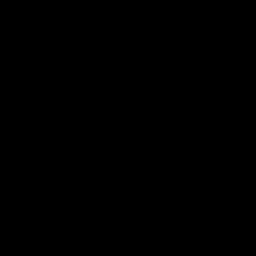
\includegraphics[height=1.5in]{images/B_m1}
        \caption{$1 \times 1$}
    \end{subfigure}%
    ~ 
    \begin{subfigure}[t]{0.24\textwidth}
        \centering
        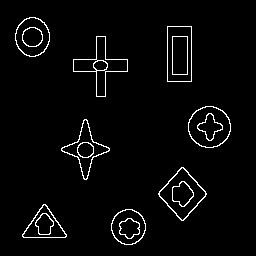
\includegraphics[height=1.5in]{images/B_m3}
        \caption{$3 \times 3$}
    \end{subfigure}%
    ~
    \begin{subfigure}[t]{0.24\textwidth}
        \centering
        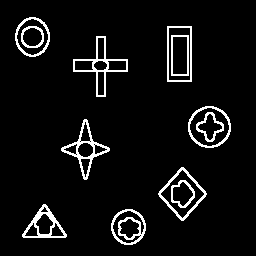
\includegraphics[height=1.5in]{images/B_m5}
        \caption{$5 \times 5$}
    \end{subfigure}%
    ~
    \begin{subfigure}[t]{0.24\textwidth}
        \centering
        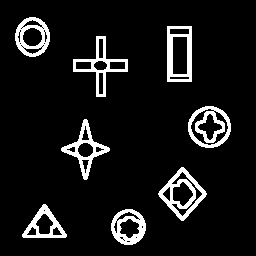
\includegraphics[height=1.5in]{images/B_m7}
        \caption{$7 \times 7$}
    \end{subfigure}
    \caption{$B$}
\end{figure}
Boundary extraction is composed of erosion and its complement
\begin{equation}
	B = I_1 \& ~(I_1 \ominus SE)
\end{equation}
where $SE$ is the structural element, square in this case.
When the sides of $SE$ increases, the more the erosion is applied on $I_1$, causing more blanked region appeared after $\& ~(I_1 \ominus SE)$, leading to thicker edges.

\subsection*{Counting objects}
The algorithm is described below 
\begin{enumerate}
\item 
Pick a non-zero pixel by scanning sequentially from the origin. Name this one pixel image as $A$. 

\item
Start from that location, dilate $A$ using structure element $SE$, a 3-by-3 square in this case.
Dilate until $A$ stops expansion, in comparison to the input image $I_1$.

\item 
Set the selected pixels in $A$ as value of $N$, a book-keeping variable, and increment $N$.

\item
Remove selected pixels in $A$ from $I_1$.

\item
Repeat this process until $I_1$ is empty.
\end{enumerate}
Though there is the possibility to modify size and shape of $SE$, since we are interesting in selecting the object, with $SE$ being too wide will certainly cause the algorithm to miss it or accidentally select its neighbor. Therefore, 3 is kept here.

\begin{figure}[H]
    \centering
    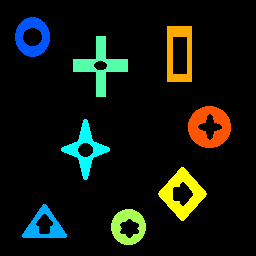
\includegraphics[height=2.5in]{images/L}
    \caption{Labeled connected components}
\end{figure}

One may consider using running length encoding to efficiently sort the result, since RLE can better utilize the cache mechanism, but two-pass is still required similar to the naive implementation provided here.

During writing of the erosion algorithm, I also found out the slide misplaced result of Sternberg and Serra definition, despite the equations themselves are correct.

\subsection*{Skeletonizing}
\begin{figure}[H]
    \centering
    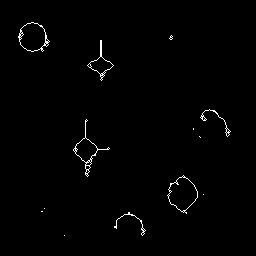
\includegraphics[height=2.5in]{images/S}
    \caption{$S$, skeletonized $I_1$}
\end{figure}
The implementation try to follow the implementation from textbook, which requires two set of lookup tables. General operation is 
\begin{equation}
	G = X \cap \lbrack \bar{M} \cup P \rbrack
\end{equation}
where $X$ is the input image, $G$ is the output image, $M$ is the conditional marker determined in the process, and $P$ is the inhibiting variable.

During the first pass, $M$ is determined by hit-and-miss transformation using the kernel from \autoref{tbl:conditional}. 
I put tons of time to figure out the decimal equivalent of them, I might as well put my result here, and there seems to be no one posting this out there on the Net.
\begin{table}[H]
\caption{Conditional}
	\centering
	\begin{tabular}{c|c}	
	Type & Decimal number \\
	\hline
	\hline
	S1 & 64, 16, 4, 1\\
	S2 & 128, 32, 8, 2\\
	S3 & 192, 96, 48, 24, 12, 6, 3, 129 \\
	TK4 & 160, 40, 10, 130 \\
	STK4 & 193, 112, 28, 7 \\
	ST5 & 176, 161, 104, 194, 224, 56, 14 ,131 \\
	ST6 & 177, 108 \\
	STK6 & 240, 225, 120, 60, 15, 135, 195 \\
	STK7 & 241, 124, 31, 199\\
	STK8 & 227, 248, 62, 143\\
	STK9 & 243, 231, 252, 249, 124, 63, 159, 207\\
	STK10 & 247, 253, 127, 223\\
	K11 & 251, 254, 191, 239\\
	\end{tabular}
	\label{tbl:conditional}
\end{table}

During the second pass, which is coined as the unconditional stage, output result is determined by combination of $X$ and $M$. 
Since there are spaces for combinations in the textbook kernel list, I separated them to three categories to ease the computation process.

\paragraph{First} type is simply equal-or-not comparison with values from \autoref{tbl:unconditional_eq}. One simply extract the surrounding pixels 
\begin{equation}
	V = \sum_{i\in\text{neighbors}}{M_i 2^i}
\end{equation}
where $V$ is the corresponding decimal value constructed by the fully connected neighbors.
Most significant bit is the first pixel, designated $M_0$ in the textbook.

\begin{table}[H]
\caption{Unconditional, EQ}
	\centering
	\begin{tabular}{c|c}	
	Type & Decimal number \\
	\hline
	\hline
	Spur & 1, 4, 64, 16\\
	4-connected & 2, 128, 8, 32\\
	L & 160, 40, 130, 10
	\end{tabular}
	\label{tbl:unconditional_eq}
\end{table}

\paragraph{Second} type requires one to provide a mask before comparison.
The comparison is composed of two parts
\begin{equation}
\begin{cases}
	P_1 = (X \vee K_M) \wedge K_C \\
	P_2 = (T \wedge \tilde{K_M}) \wedge (K_C \wedge \tilde{K_M})\\
\end{cases}
\label{eq:unconditional_or_eq_eq}
\end{equation}
and the final result is determined by 
\begin{equation}
	P = P_1 \wedge P_2
\end{equation}
$P_1$ used the mask to ignore flexible $D$ terms in the table provided in the textbook, while $P_2$ verifies the constant terms, $M$, $0$ and $1$ are satisfied as well.
$K_M$ is the mask while $K_C$ is the conditional equivalent decimal number, both of them are enlisted as a pair $(K_M, K_C)$ in \autoref{tbl:unconditional_or_eq}.

\begin{table}[H]
\caption{Unconditional, OR-EQ}
	\centering
	\begin{tabular}{c|c}	
	Type & (Mask, Condition) \\
	\hline
	\hline
	Corner & (31, 255), (241, 255), (199, 255), (124, 255) \\
	Tee & (84, 252), (213, 255), (117, 255), (93, 255) \\
	Diagonal & (17, 181), (68, 109), (17, 91), (68, 214)\\
	\end{tabular}
	\label{tbl:unconditional_or_eq}
\end{table}

\paragraph{Third} type is similar to the second type, but instead of equivalent, it requires unequal, since in the textbook, 
\begin{equation}
	A \cup B \cup C = 1
\end{equation}
in other words, one of them has to be 1, complementary is relatively easy to test for.

Under this consensus, \autoref{eq:unconditional_or_eq_eq} can be modified as
\begin{equation}
\begin{cases}
	P_1 = \sim ((X \vee K_M) \vee K_C) \\
	P_2 = (T \wedge \tilde{K_M}) \wedge (K_C \wedge \tilde{K_M})\\
\end{cases}
\label{eq:unconditional_or_eq_eq}
\end{equation}

\begin{table}[H]
\caption{Unconditional, OR-NEQ}
	\centering
	\begin{tabular}{c|c}	
	Type & (Mask, Condition) \\
	\hline
	\hline
	Vee & (184, 248), (42, 62), (138, 143), (162, 227) \\
	\end{tabular}
\end{table}

If short segments are unwanted, pruning algorithm can be employed. In my implementation, some objects seem to being thinned too aggressively, however, I haven't found the pitfalls in the pipeline for the time being. 

\end{document}
              